\documentclass{beamer}

%-----------------------------------------------------------------
\usepackage{lmodern}

\usepackage[latin1]{inputenc}
\usepackage{xcolor}
\usepackage{fontenc}

\usepackage{latexsym}
\usepackage{amsmath,amsthm,amssymb,color, bm}
\usepackage{array}
\usepackage{enumerate}

\usepackage{multirow,multicol,tabu}
 
% using for \coloneqq and \span
\usepackage{mathtools}
 



%===============================================================


\begin{document}

%=================================================================
\begin{frame}
\frametitle{Title of the frame}

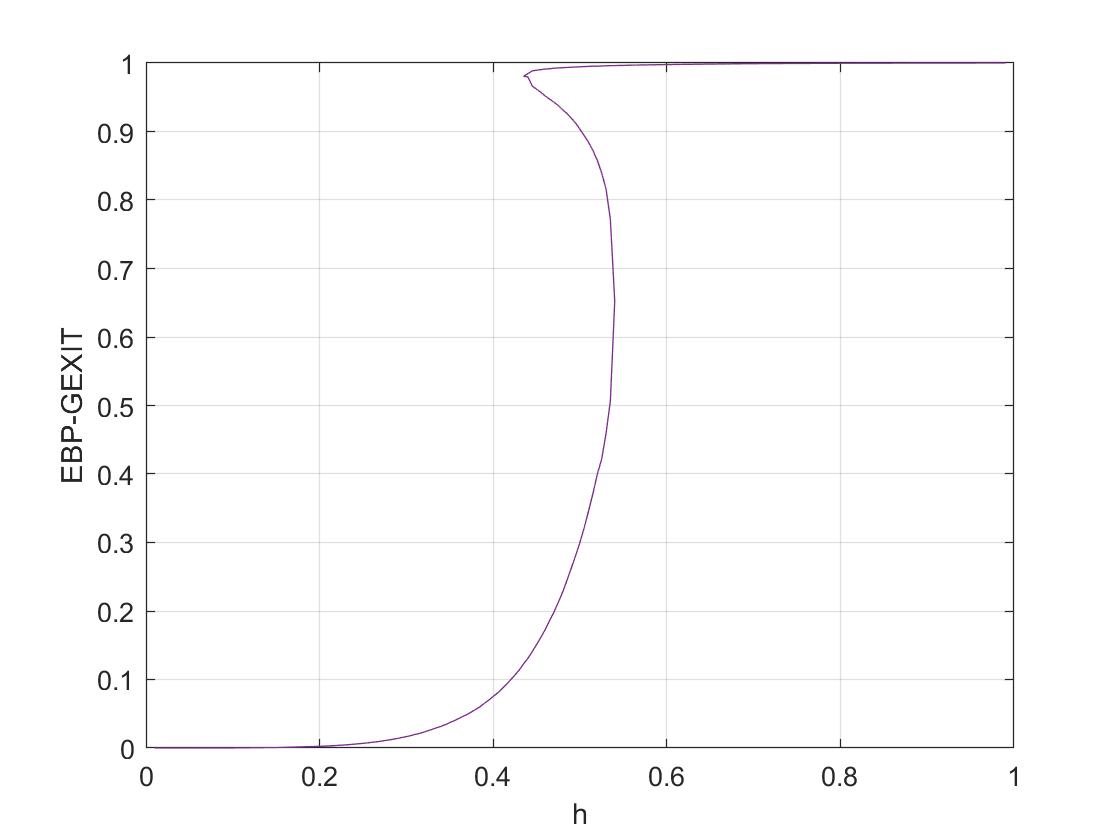
\includegraphics[width=0.5\textwidth]{Sample_figure.jpg}

\begin{itemize}
% 
\item Item 1
% 
\pause
% 
\item \textcolor{red}{Item 2}
%  
\end{itemize}

\begin{align}
%  
x = y + z
% 
\end{align}


 
\end{frame}


\end{document}



